\documentclass[11pt]{article}
\usepackage[T1]{fontenc}
\usepackage{lmodern}
\usepackage[margin=0.92in]{geometry}
\usepackage{amsmath,amssymb,amsthm,mathtools}
\usepackage{microtype,booktabs,array}
\usepackage{tikz}
\usepackage[hidelinks]{hyperref}
\pdfinfoomitdate=1
\pdftrailerid{}
\pdfsuppressptexinfo=15
\hypersetup{pdftitle={Incoming preparation constraints and quadratic source budgets for scalar shells},
 pdfauthor={Ricardo Maldonado},pdfsubject={Working manuscript for author and specialist review}}
\newcommand{\dd}{\,\mathrm d}
\newcommand{\eps}{\varepsilon}
\newcommand{\HH}{H}
\newcommand{\PN}{P_{\!N}}
\newcommand{\PD}{P_{\!D}}
\newcommand{\ip}[2]{\langle #1,#2\rangle_H}
\newcommand{\norm}[1]{\lvert #1\rvert_H}
\newcommand{\calV}{\mathcal V}
\newcommand{\Dmat}{D_{\mathrm{op}}}
\newtheorem{proposition}{Proposition}
\newtheorem{assumption}{Retained premise}
\newtheorem{remark}{Remark}
\title{Incoming preparation constraints and quadratic source budgets for scalar shells}
\author{Ricardo Maldonado\\Independent Researcher}
\date{4 November 2026\\[3pt]\small Working manuscript for author and specialist review}
\begin{document}
\maketitle
\begin{abstract}
We distinguish a prescribed present perturbation from an incoming physical
preparation for a five-dimensional Einstein--scalar shell. The registered
compact master packet has nonzero velocity and both principal characteristic
channels; their normalized imbalance is at most $\ell^2/4$ for
$\ell=10^{-6}$. This diagnostic neither identifies a physical energy flux nor
excludes an incoming past state that subsequently scatters.
For the actual first canonical jet, a tilted five-channel energy gives a
conditional continuous source-to-shell estimate with growth rate $301/100$.
Integrating retained quadratic source bounds over five clipped cells of total
area $9/32$ yields an exact source ledger. Its zero-initial-data trace bound
is auxiliary, weaker than a retained direct estimate, and does not supply a
constraint-compatible physical second state.
On a separately declared past affine null cut, the Raychaudhuri constraint
determines an explicit nonpositive second expansion and logarithmic area
response after free second scalar data and corner constants are fixed.
Actual second area has an additional nonnegative first-variation square.
A restricted inverse estimate also identifies admissible present preparations
from a normalized physical scalar history. None of these statements selects
a past state, a preparation radius, a matter-production mechanism, or a
cosmological origin.
\end{abstract}

\section{Preparation question and retained model}
An initial perturbation on a supplied Cauchy slice does not specify how that
state was prepared. This distinction is especially relevant at second order:
the first perturbation fixes quadratic bulk and junction sources, while the
second constraints still permit additional homogeneous data. Previous
preparation comparisons for this model control shell-volume differences on
a restricted canonical fiber by a geometric initial profile and its $H^1$
norm~\cite{geometric,h1}. Here we ask what an incoming prescription would
have to add. The results are a present-packet diagnostic, an actual-source
ledger, one solved null constraint, and an inverse estimate on an admissible
present-state image. They are not a construction of the full past problem.

We retain the action normalization
\begin{equation}
 S_{\rm bulk}=\int_{\mathcal M}\!
 \left(\frac{R}{2}-\frac{|\nabla\phi|^2}{2}-V(\phi)\right)\dd\mu_g,
 \qquad
 {\rm Ric}_{AB}=\partial_A\phi\,\partial_B\phi+\frac23Vg_{AB},
 \quad \Box_g\phi=V'(\phi).
 \label{eq:action}
\end{equation}
Two identical interiors meet at a pure-tension shell. In the retained
outward-normal convention their one-copy laws are
\begin{equation}
 K^{\rm out}_{\mu\nu}=\frac{\sigma}{6}\gamma_{\mu\nu},
 \qquad n_{\rm out}\phi=-\frac{\sigma'}2.
 \label{eq:junction}
\end{equation}
The fixed model uses
\begin{equation}
\begin{aligned}
 W(\phi)&=1-\phi+\frac{\phi^3}{3},&
 V&=\frac{(W')^2}{2}-\frac{2W^2}{3},\\
 \sigma(\phi)&=2W(\phi)+10^{-3}(1+c_\sigma\phi),&
 c_\sigma&=\frac{96714321425692}{161839258930731}.
\end{aligned}
\label{eq:model}
\end{equation}
Let $\kappa$ be the unit three-sphere metric. The retained spherical
background has
\begin{equation}
 g_0=\dd y^2+\rho(y)^2[-\dd t^2+\cosh^2t\,\kappa]
     =\rho(z)^2[-\dd t^2+\dd z^2+\cosh^2t\,\kappa],
 \quad \dd y=-\rho\dd z.
 \label{eq:background}
\end{equation}
The shell is $z=0$, $\rho_b=\rho(0)$, $a=\rho_y/\rho$, and
$p=\phi_{0,y}\ne0$ on the collar in use. Set
\begin{equation}
 \ell=10^{-6},\qquad x=t/\ell,\qquad r=z/\ell,\qquad
 T=\frac54,\qquad \tau_*=\rho_b\ell T.
 \label{eq:scales}
\end{equation}
All estimates below use this fixed model normalization; no measured SI units
are assigned. A subscript $j$ denotes the actual derivative
$\partial_\eps^j|_{\eps=0}$, so a second perturbation enters a Taylor series
as $\eps^2 X_2/2$.

\begin{assumption}
The background, the common first packet, the retained analytic reductions,
the regular exact-family and uniqueness premises, and the continuous
future-cone operator caps stated in Section~\ref{sec:energy} are shared
inputs. The present calculation does not reprove them. In particular,
finite source certificates do not by themselves prove a coefficient bound
at every point.
\end{assumption}
The physical slice, shell anchor, scalar-level component, and background
scalar labels used in the earlier geometric preparation class remain
supplied structure. A new past prescription must establish a compatible
development before it can be tested against that class.

\section{The actual first packet and its two principal channels}
\label{sec:packet}
The registered master data are
\begin{equation}
\begin{aligned}
 w(0,z)&=q_\ell(z),& w_t(0,z)&=e^{-z}q_\ell(z),\\
 q_\ell(z)&=
 \begin{cases}
 \exp\!\left(4-\dfrac{\ell^2}{(z-\ell)(2\ell-z)}\right),&
                  \ell<z<2\ell,\\
 0,&\text{otherwise}.
 \end{cases}
\end{aligned}
\label{eq:packet}
\end{equation}
The function is smooth and flat at both endpoints. In scaled variables
$W_0=Q(r)=q_\ell(\ell r)$ and $W_{x,0}=\ell e^{-\ell r}Q$.
At $r=3/2$, $Q=1$ and $Q_r=0$, so both
$W_x+W_r$ and $W_x-W_r$ are strictly positive. Background time symmetry,
$K_0=\Pi_0=0$, does not make this perturbation time symmetric.

The first physical metric and scalar data are reconstructed together.
Writing $\mathcal Y=n_1^2-n_2^2$ on the unit three-sphere, define
\begin{equation}
\begin{aligned}
 \alpha&=(\rho/\rho_b)^{3/2}p/p_b,&
 C&=\alpha/\rho^2,& B&=3\alpha/(\rho^3p),\\
 k_{\rm bg}&=\rho(5a/2-V'/p),&
 u&=Cq_\ell,&v&=B(q_{\ell,z}+k_{\rm bg}q_\ell).
\end{aligned}
\end{equation}
Their actual velocities, not freely assigned zero velocities, are
\begin{equation}
 u_t=e^{-z}u,\qquad
 v_t=e^{-z}\!\left(v-\frac{3u}{\rho p}\right)
     =Be^{-z}\big[q_{\ell,z}+(k_{\rm bg}-1)q_\ell\big].
 \label{eq:velocities}
\end{equation}
In radial/angular orthonormal order the Cauchy data are
\begin{equation}
\begin{aligned}
 \gamma_1&=\operatorname{diag}(-4u,2u,2u,2u)\mathcal Y,\\
 K_1&=\rho^{-1}\operatorname{diag}(-2u_t,u_t,u_t,u_t)\mathcal Y,
 &\phi_1&=v\mathcal Y,&\Pi_1&=v_t\mathcal Y/\rho.
\end{aligned}
\label{eq:firstdata}
\end{equation}
For the convention
$\pi^{ij}=\sqrt\gamma(K^{ij}-K\gamma^{ij})/2$, these imply
\begin{equation}
 \frac{\pi_1}{\sqrt{\gamma_0}}
 =\operatorname{diag}\!\left(-\frac{3u_t}{2\rho},0,0,0\right)\mathcal Y,
 \qquad \frac{\varpi_1}{\sqrt{\gamma_0}}=\Pi_1.
 \label{eq:canonical}
\end{equation}
Harmonic completion further fixes
\begin{equation}
\begin{aligned}
 N_1&=\rho u\mathcal Y,&\beta_1&=0,&
 \dot N_1&=\rho u_t\mathcal Y,\\
 \dot\beta_1^y&=-6\rho^2(u_y+4au)\mathcal Y,&
 \dot\beta_1^a&=0\quad(a=1,2,3),&
 \dot\gamma_1&=2\rho K_1,\quad\dot\phi_1=v_t\mathcal Y.
\end{aligned}
\label{eq:harmonic}
\end{equation}
The quadratic sources used below are joined to this complete canonical and
harmonic one-jet. The retained 31 October velocity correction concerned a
\emph{second-response approximation}; it did not replace
\eqref{eq:packet} by time-symmetric first data.

For a transparent principal-part diagnostic, introduce
\begin{equation}
 E_\pm=\frac14\int_\ell^{2\ell}(e^{-z}q_\ell\pm q_{\ell,z})^2\dd z.
 \label{eq:weights}
\end{equation}
These positive quadratic weights refer to the normalized master, not to a
physical Noether energy or a measured incoming flux. Integration by parts
using flat endpoints gives
\begin{equation}
\begin{aligned}
 E_+-E_-&=\int e^{-z}q_\ell q_{\ell,z}\dd z
          =\frac12\int e^{-z}q_\ell^2\dd z>0,\\
 E_++E_-&=\frac12\int(q_{\ell,z}^2+e^{-2z}q_\ell^2)\dd z,\\
 \delta:=\frac{E_+-E_-}{E_++E_-}
 &=\frac{\int e^{-z}q_\ell^2\dd z}
         {\int(q_{\ell,z}^2+e^{-2z}q_\ell^2)\dd z}
 \le\frac{\ell^2}{4}=\frac1{4000000000000}.
\end{aligned}
\label{eq:imbalance}
\end{equation}
Indeed, endpoint Cauchy--Schwarz gives
$|f(z)|^2\le\min(z-\ell,2\ell-z)\int|f'|^2$ for a function
vanishing at both endpoints. Its integral bounds $\int f^2$ by
$\ell^2\int(f')^2/4$. Since $e^{-z}\le1$, this proves the last line without
new bump evaluations. The normalized weights are $(1\pm\delta)/2$:
each differs from $1/2$ by at most $1/8000000000000$.

For the free principal part, $W_x+W_r$ propagates toward the shell,
whereas $W_x-W_r$ propagates away. Pure propagation toward the shell now
would require $Q_r=\ell e^{-\ell r}Q$; its zero endpoint value forces the
zero solution, contrary to \eqref{eq:packet}. The opposite one-way condition
also fails. The actual equation includes a potential and a reflecting,
coupled shell. Thus these present data may in principle result from an
incoming past state after scattering. The calculation establishes neither
that history nor its impossibility.

\section{Forced mean equations and the physical corner}
\label{sec:forced}
Use the retained five mean fields $U=(K,L,N,J,w)$ with
$H=\operatorname{diag}(1,2,1,3,1)$. Let $\PD$ project onto $L$ and
$\PN=1-\PD$; these projections are orthogonal in $H$. The actual second
mean equations on the future cone are
\begin{equation}
\begin{aligned}
 U_{xx}-U_{rr}&=A U_x+B U_r+\Dmat U+S_0,\\
 \PD U&=0,\qquad \PN U_r=M u+G_0,\qquad
 u=\PN U(x,0).
\end{aligned}
\label{eq:forced}
\end{equation}
The boundary derivative in \eqref{eq:forced} points toward
\emph{increasing $r$}, away from the shell. In terms of the quadratic
reduced Einstein, scalar, and one-copy junction Hessians, the adapters are
\begin{equation}
\begin{aligned}
 S_0&=P_0(-2\ell^2\rho^2 Q_{E,\mathrm{red}},\;\ell^2\rho^2 Q_\phi),\\
 G_0&=\ell\rho_b(-G_{N,0},\,0,\,2Q_{R00,0},\,
                         2Q_{RJ,0},\,Q_{P,0}),\\
 G_{N,0}&=2Q_{R00,0}-6Q_{RJ,0}-2Q_{Cy,0}.
\end{aligned}
\label{eq:adapters}
\end{equation}
Here $P_0$ is angular mean projection, $Q_{RJ,0}$ is the mean angular
junction row, and the subscript $0$ on a source row denotes that projection,
not a vanishing source. The sign uses $\partial_r=-\ell\rho\partial_y$.
The source is a derivative forcing in the Robin law, not its time integral.
There is no additional factor $1/2$ in these actual-second-variation
adapters.

For example, in the geometric shell Hessian map write first normal lapse
$H_f=A_f\mathcal Y$, induced components
$m_{00}=D_f\mathcal Y$ and
$m_{ab}=L_f\mathcal Y\kappa_{ab}+M_f\nabla_a\nabla_b\mathcal Y$,
and scalar $\eta=s_f\mathcal Y$. With
\begin{equation}
\begin{aligned}
 c_f&=aA_f^2/4-\sigma'A_fs_f/6-\sigma''s_f^2/6,\\
 d_f&=aA_f+\sigma's_f/3,\qquad
 q_f=pA_f^2/4+\sigma''A_fs_f/2+2s_f^2,
\end{aligned}
\end{equation}
the retained angular moments give
\begin{equation}
 Q_{R00,0}=\frac{-c_f-d_fD_f}{6},\quad
 Q_{RJ,0}=\frac{c_f-d_fL_f}{6}+\frac{4d_fM_f}{9},
 \quad Q_{P,0}=\frac{q_f}{6}.
\end{equation}
Together with the Codazzi row, this records which geometric source is being
bounded; it does not substitute a test scalar for the actual metric jet.

Set $J_\pm=U_x\pm U_r$. The characteristic and shell identities are exactly
\begin{equation}
\begin{aligned}
 (\partial_x\mp\partial_r)J_\pm&=A U_x+B U_r+\Dmat U+S_0,\\
 \PN J_-&=\PN J_+-2(Mu+G_0),\\
 u_x&=\PN J_+-Mu-G_0,\qquad \PD J_-=-\PD J_+.
\end{aligned}
\label{eq:char}
\end{equation}
Thus a shell incoming characteristic combination cannot be prescribed
independently while keeping the junction condition fixed.
At a regular Cauchy--shell corner, with $U_0=U(0,\cdot)$ and
$V_0=U_x(0,\cdot)$, one must have
\begin{equation}
\begin{aligned}
 \PD U_0=\PD V_0&=0,\qquad
 \PN U_{0,r}=M(0)u_0+G_0(0),\\
 \PN V_{0,r}&=M_x(0)u_0+M(0)\PN V_0+G_{0,x}(0).
\end{aligned}
\label{eq:corner}
\end{equation}
Higher regularity imposes further differentiated identities. The actual
packet has an open background collar at the initial shell: the needed
source and data jets vanish there. This verifies these corner rows for the
retained packet. It does not verify a corner for a newly chosen past state.

\section{A continuous tilted energy with actual forcing}
\label{sec:energy}
On $0\le r\le T-x$ put $V=U_x$, $P=U_r$, $k=\alpha=1/2$, and
\begin{equation}
 e=\frac{\norm{V}^2+\norm{P}^2+2k\ip{V}{P}+\norm{U}^2}{2},
 \qquad
 E(x)=\int_0^{T-x}e(x,r)\dd r+\frac{\alpha}{2}\norm{u(x)}^2.
 \label{eq:energy}
\end{equation}
The cross term is a standard tilted wave energy device~\cite{wave}.
It is positive since $|k|<1$; it is not identified here with a physical
Noether energy or a preparation law.
The retained continuous operator bounds, in the $H$-induced norm, are
\begin{equation}
 \|A\|,\|B\|\le10^{-4},\qquad
 \|\Dmat\|\le10^{-6},\qquad \|M\|\le\mu:=\frac1{2000}.
 \label{eq:caps}
\end{equation}
They are conditional analytic premises on the existing future cone.
They are not new all-point proofs, and give no cap on a new past domain
or for a different first state.

\begin{proposition}
Under \eqref{eq:caps}, every regular solution of \eqref{eq:forced}
satisfies, including the zero-energy case,
\begin{equation}
 E'(x)\le\frac{301}{100}E(x)
 +\frac12\|S_0(x,\cdot)\|_{L^2(H)}^2
 +\frac{5002001}{4000000}\norm{G_0(x)}^2.
 \label{eq:forcedenergy}
\end{equation}
No selfadjointness, positivity, or time independence of $M$ is required.
\end{proposition}
\begin{proof}
With $F=AV+BP+\Dmat U$, direct differentiation gives
$e_x=f_r+\ip{V+kP}{F+S_0}+\ip{U}{V}$, where
$f=\ip{V}{P}+k(\norm{V}^2+\norm{P}^2)/2$.
For $a_*=b_*=10^{-4}$ and $d_*=10^{-6}$, the homogeneous bulk
production is at most $c_V\norm{V}^2+c_P\norm{P}^2+c_U\norm{U}^2$, with
\begin{align*}
 c_V&=a_*+(b_*+ka_*)/2+d_*/2+1/2,\\
 c_P&=kb_*+(b_*+ka_*)/2+kd_*/2,\qquad
 c_U=d_*/2+kd_*/2+1/2.
\end{align*}
Its rate is bounded by
$\max\{2c_V/(1-k),2c_P/(1-k),2c_U\}=2.000702$.
At the homogeneous Robin boundary, put $j=\PN(V+P)$ and
$\gamma_*=\alpha+(1-k)\mu$. Completing one square gives
\[
 -f_N+\alpha\ip{u}{\PN V}
 \le-\frac{k}{4}\norm{j}^2+
 \left[\frac{\gamma_*^2}{k}+(1-k)\mu^2+\alpha\mu\right]\norm{u}^2.
\]
The coefficient relative to the boundary energy is $2.003001$.
This leaves $-\norm{j}^2/8$ available for absorption.
The moving outer flux is
\[
 -\frac{1-k}{2}\norm{V-P}^2-\frac12\norm{U}^2\le0,
\]
and the physical Dirichlet contribution is nonpositive. These conclusions
follow by direct integration by parts for this mixed boundary problem;
they are not an application of a theorem assuming a different boundary law.

For the bulk forcing one has the exact square identity
\[
 2e-\norm{V+kP}^2=(1-k^2)\norm{P}^2+\norm{U}^2\ge0.
\]
Consequently
$\ip{V+kP}{S_0}\le e+\norm{S_0}^2/2$, adding at most one to the
bulk rate. Expanding the Robin boundary expression about its homogeneous
value adds exactly
\[
 -\tfrac12\ip{j}{G_0}+\ip{Mu}{G_0}
       +\tfrac12\norm{G_0}^2-\tfrac12\ip{u}{G_0}.
\]
Use the reserved negative square and then Young's inequality:
\begin{align*}
 -\norm{j}^2/8+\norm{j}\norm{G_0}/2&\le\norm{G_0}^2/2,\\
 (\mu+1/2)\norm{u}\norm{G_0}
 &\le\norm{u}^2/4+(\mu+1/2)^2\norm{G_0}^2.
\end{align*}
The first term in the second line is exactly the boundary summand in
$E$. Thus the total boundary source coefficient is
$1+(\mu+1/2)^2=5002001/4000000$. Both enlarged homogeneous rates are
below $301/100$, proving \eqref{eq:forcedenergy}.
\end{proof}

With $C=301/100$ and $C_G=5002001/4000000$, integration gives
\begin{equation}
\begin{aligned}
 E(x)\le e^{Cx}E(0)+\int_0^x e^{C(x-s)}
 \left[\frac12\|S_0(s,\cdot)\|_{L^2(H)}^2
                  +C_G\norm{G_0(s)}^2\right]\dd s,\\
 e^{CT}=e^{301/80}<44,\qquad
 |w(x,0)|^2\le\norm{u(x)}^2\le4E(x).
\end{aligned}
\label{eq:convolution}
\end{equation}
The exponential upper bound follows from a rational Taylor sum and a
geometrically bounded tail. The estimate retains the coupled metric,
scalar, and nonselfadjoint Robin feedback. It does not assume that a
single uncoupled scalar energy controls the other fields.

\section{The clipped source ledger and its interpretation}
\label{sec:ledger}
The retained actual-jet certificates give global source bounds
\begin{equation}
 F_H=17387513156573,\qquad G_H=3851400.
 \label{eq:globalcaps}
\end{equation}
The future cone is $x\ge0$, $r\ge0$, $x+r\le T$, of area $25/32$.
Finite propagation and the open initial collar give the exact zero wedge
$x+r\le1$. Hence the active bulk has area $9/32$, and the active shell
segment is $1\le x\le5/4$, of length $1/4$.
The old half-unit certificate grid intersects the active cone in five
nonempty polygons, shown in Figure~\ref{fig:cells}. Integrating each
retained cell cap only over its clipped polygon avoids a new source call.

\begin{figure}[htbp]
\centering
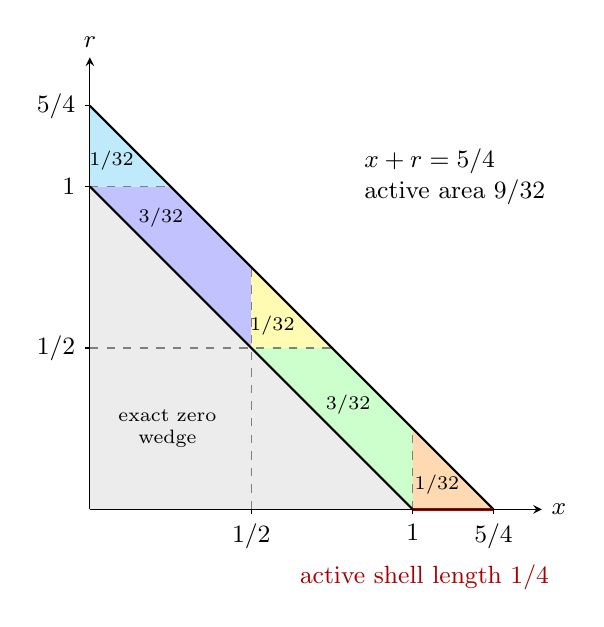
\begin{tikzpicture}[scale=4.1,>=stealth,font=\small]
 \fill[gray!15] (0,0)--(1,0)--(0,1)--cycle;
 \fill[blue!24] (0,1)--(.25,1)--(.5,.75)--(.5,.5)--cycle;
 \fill[cyan!25] (0,1)--(0,1.25)--(.25,1)--cycle;
 \fill[green!20] (.5,.5)--(.75,.5)--(1,.25)--(1,0)--cycle;
 \fill[yellow!30] (.5,.5)--(.5,.75)--(.75,.5)--cycle;
 \fill[orange!30] (1,0)--(1,.25)--(1.25,0)--cycle;
 \draw[gray,dashed] (.5,0)--(.5,.75) (1,0)--(1,.25)
                         (0,.5)--(.75,.5) (0,1)--(.25,1);
 \draw[thick] (0,1)--(1,0) (0,1.25)--(1.25,0);
 \draw[very thick,red!65!black] (1,0)--(1.25,0);
 \draw[->] (0,0)--(1.40,0) node[right] {$x$};
 \draw[->] (0,0)--(0,1.40) node[above] {$r$};
 \foreach \a/\lab in {.5/{1/2},1/{1},1.25/{5/4}} {
  \draw (\a,0)--(\a,-.015) node[below] {$\lab$};
  \draw (0,\a)--(-.015,\a) node[left] {$\lab$};}
 \node[align=center,font=\scriptsize] at (.24,.25) {exact zero\\wedge};
 \node[font=\scriptsize] at (.22,.905) {$3/32$};
 \node[font=\scriptsize] at (.067,1.08) {$1/32$};
 \node[font=\scriptsize] at (.80,.325) {$3/32$};
 \node[font=\scriptsize] at (.565,.57) {$1/32$};
 \node[font=\scriptsize] at (1.075,.075) {$1/32$};
 \node[anchor=west,align=left] at (.82,1.03)
 {$x+r=5/4$\\active area $9/32$};
 \node[anchor=west,red!65!black] at (.62,-.21)
 {active shell length $1/4$};
\end{tikzpicture}
\caption{Clipping the retained half-unit cells to
$1<x+r\le5/4$. Labels are exact polygon areas; cell boundaries are dashed.
The red shell segment carries the active Robin source.
This is a source-integration domain, not a new past development.}
\label{fig:cells}
\end{figure}

Let
\begin{equation}
 I_{\rm bulk}=\int_0^T\|S_0(x,\cdot)\|_{L^2(H)}^2\dd x,\quad
 I_{\rm bd}=\int_0^T\norm{G_0(x)}^2\dd x,\quad
 B_{\rm src}=\frac12 I_{\rm bulk}+C_G I_{\rm bd}.
\end{equation}
Exact rational integration of the retained cell caps gives the outward
integer bounds
\begin{equation}
\begin{aligned}
 I_{\rm bulk}&\le 8526418129275428520152526,\\
 I_{\rm bd}&\le 3708320490000,\\
 B_{\rm src}&\le4263209064642351515776089.
\end{aligned}
\label{eq:ledgerintegers}
\end{equation}
For comparison, using only the active area and the global cap gives
$I_{\rm bulk}\le9F_H^2/32<8.50291\,10^{25}$; the cell integration
gives $I_{\rm bulk}<8.52642\,10^{24}$.
The source amplitudes were retained rather than newly sampled.
The arithmetic authenticates the selected old inputs and integrates their
enclosures; it does not reconstruct the quadratic source function.

Equations~\eqref{eq:convolution}--\eqref{eq:ledgerintegers} imply
\begin{equation}
 |w(x,0)|^2\le176\bigl(E(0)+B_{\rm src}\bigr).
 \label{eq:trace}
\end{equation}
For the \emph{auxiliary} forced problem with $U_0=V_0=0$, this yields
\begin{equation}
 \sup_{0\le x\le T}|w(x,0)|\le27392057158547.
 \label{eq:aux}
\end{equation}
This is not an improved numerical response prediction: the retained direct
Duhamel estimate of about $5.4\,10^{12}$ is smaller.
The purpose of \eqref{eq:aux} is a continuous, source-norm-based ledger.

Crucially, the auxiliary zero state is not a physical zero second
Einstein--scalar state. The second constraints read
$P X_2=-D^2{\cal C}[X_1,X_1]$. For the actual packet the retained
Hamiltonian Hessian witness is less than $-10^{19}$ at its center.
Setting \emph{all} second Cauchy fields to zero therefore fails that
constraint. An affine seed before solving the constraints is a different
object. Nor does a bound on $w$ alone omit the common first-quadratic
proper-clock, volume-measure, and Gauss terms required for an absolute
shell-volume or shell-expansion coefficient.

\section{A declared past cut and its forced null constraint}
\label{sec:null}
\subsection{Affine geometry and background check}
One candidate past initial characteristic surface is the
\emph{outgoing-relative-to-the-shell} cut
\begin{equation}
 {\cal C}_-=\{t-z=t_-\},\qquad t_-<-2\ell,
 \label{eq:cut}
\end{equation}
restricted to a segment of the actual positive collar preceding $t=0$.
Its shell corner is $(t_-,0)$. The strict margin matters for encompassing
the present packet. An incoming pulse crossing this outgoing cut could
later move toward the shell; the cut orientation is not the pulse direction.
A future affine background generator is
\begin{equation}
 k_0=c\rho^{-2}(\partial_t+\partial_z),\qquad c>0,
 \qquad R_0(\lambda)=\rho(z(\lambda))\cosh t(\lambda).
 \label{eq:generator}
\end{equation}
It increases $z$ away from the shell. The positive constant $c$ must be fixed
by a declared corner-clock normalization. Primes in this section mean
affine $\lambda$ derivatives. The background screen has dimension three,
and its expansion and scalar derivative are
\begin{equation}
 \vartheta_0=3R_0'/R_0
       =3c\rho^{-2}(\tanh t-\rho a),\qquad
 \Phi_0'=-cp/\rho.
 \label{eq:theta0}
\end{equation}
In particular, the screen radius is not $\rho$ alone.

An exact background check fixes the signs and normalization.
The static equations imply
$\rho_z=-a\rho^2$, $a_y=-1/\rho^2-p^2/3$, and hence
$a_z=1/\rho+\rho p^2/3$. Put $A_0=\rho a$, $T_0=\tanh t$,
and $\partial_+=\partial_t+\partial_z$. Then
\[
 \partial_+(T_0-A_0)=A_0^2-T_0^2-\rho^2p^2/3,\qquad
 \partial_+(\rho^{-2})=2A_0\rho^{-2}.
\]
Substituting in \eqref{eq:theta0} cancels every $A_0,T_0$ term in
$\vartheta_0'+\vartheta_0^2/3$, leaving
$-c^2p^2/\rho^2=-(\Phi_0')^2$. This algebraic identity does not
constitute a numerical enclosure on a new past domain.

For a smooth family, choose physical null cuts $ {\cal C}_\eps$ and pull
them back to fixed $(\lambda,\omega)$ so that
$k_\eps=\partial_\lambda$ is affine for every family member with the
specified corner normalization. Both the embedding and the normalization
belong to the new state prescription. Let $q_{\eps,AB}$ be the positive
screen metric and $\Phi_\eps$ the pulled-back scalar. Define
\begin{equation}
 {\cal B}_{AB}=\frac12q_{AB}',\qquad
 \vartheta=q^{AB}{\cal B}_{AB},\qquad
 \varsigma_{AB}={\cal B}_{AB}-\frac{\vartheta}{3}q_{AB}.
\end{equation}
Twist vanishes because the cut is a null hypersurface.
At the background $q_0=R_0^2\kappa$ and $\varsigma_0=0$.
The coefficients $\Phi_j$ include cut and generator changes through the
pullback. An old harmonic-coordinate scalar coefficient cannot be
substituted without performing that transport.

\subsection{Second expansion and logarithmic area}
For \eqref{eq:action}, $ {\rm Ric}(k,k)=(\Phi')^2$ since the potential term
vanishes on a null vector. The affine optical constraint is
\begin{equation}
 \vartheta'+\frac{\vartheta^2}{3}
          +|\varsigma|_q^2+(\Phi')^2=0.
 \label{eq:raych}
\end{equation}
Its first and actual second variations are
\begin{align}
 \vartheta_1'+\frac{2\vartheta_0}{3}\vartheta_1
       &=-2\Phi_0'\Phi_1',\label{eq:raych1}\\
 \vartheta_2'+\frac{2\vartheta_0}{3}\vartheta_2
       &=-\frac23\vartheta_1^2-2|\varsigma_1|_{q_0}^2
                  -2(\Phi_1')^2-2\Phi_0'\Phi_2'.
 \label{eq:raych2}
\end{align}
No $\varsigma_2$ term or extra inverse-metric term survives at this order
because $\varsigma_0=0$. The factors two follow from actual second
variation. The fixed affine pullback is essential: a changing nonaffine
generator would introduce additional terms.

The integrating factor in \eqref{eq:raych2} is $R_0^2$. Thus generally
\begin{equation}
\begin{aligned}
 R_0(\lambda)^2\vartheta_2(\lambda)
 &=R_0(\lambda_0)^2\vartheta_2(\lambda_0)\\
 &\quad-2\int_{\lambda_0}^{\lambda}R_0(s)^2
 \left[\frac{\vartheta_1^2}{3}+|\varsigma_1|^2
                 +(\Phi_1')^2+\Phi_0'\Phi_2'\right](s)\dd s.
\end{aligned}
\label{eq:generalnull}
\end{equation}
The mixed scalar term has no fixed sign. Now \emph{declare} the candidate
free-state and corner conditions
\begin{equation}
 \Phi_2=0\quad\hbox{on }{\cal C}_-,\qquad
 \vartheta_2(\lambda_0,\omega)=0.
 \label{eq:newstate}
\end{equation}
These are new assumptions, not consequences of the action or equivalent
to zero scalar second data on the present Cauchy slice. Define
$S_1=\vartheta_1^2/3+|\varsigma_1|^2+(\Phi_1')^2\ge0$.
Then the unique response of this constraint is
\begin{equation}
 \vartheta_2(\lambda,\omega)
 =-2R_0(\lambda)^{-2}
      \int_{\lambda_0}^{\lambda}R_0(s)^2S_1(s,\omega)\dd s\le0.
 \label{eq:nullsign}
\end{equation}
It is strictly negative downstream of a positive integral.
The first expansion is itself constrained by \eqref{eq:raych1};
it is not assignable independently of the first scalar data.

Write $ {\cal L}_\eps=\log(\dd\mu_{q_\eps}/\dd\mu_{q_0})$.
Since $ {\cal L}_j'=\vartheta_j$, the additional corner choice
$ {\cal L}_2(\lambda_0)=0$ gives
\begin{equation}
 {\cal L}_2(\lambda,\omega)
 =-2\int_{\lambda_0}^{\lambda}R_0(s)^2S_1(s,\omega)
       \left[\int_s^\lambda R_0(v)^{-2}\dd v\right]\dd s\le0.
 \label{eq:logarea}
\end{equation}
Actual area is different. At a fixed affine section,
\begin{equation}
 \frac{A_2(\lambda)}{A_0(\lambda)}
       =\left\langle{\cal L}_2+{\cal L}_1^2\right\rangle_\kappa.
 \label{eq:actualarea}
\end{equation}
The nonnegative square prevents an actual-area sign conclusion from
\eqref{eq:logarea} alone. Moreover $\vartheta_2$ is not the proper-time
shell expansion $\Theta_2$, and these null sections are not the
scalar-level sections on a physical Cauchy slice used in the geometric
profile $D$. Relating them requires clock, embedding, scalar-label,
and canonical transport.

\subsection{Extent of the construction}
Equations~\eqref{eq:generalnull}--\eqref{eq:logarea} solve one necessary
null Einstein constraint once free data and corner constants are supplied.
They do not solve the remaining null constraints, the scalar wave equation,
the shell junction law, or a nonlinear characteristic initial/boundary
problem. The present mixed packet does not already provide its first
$\Phi_1,\varsigma_1$ on this past cut. Obtaining them requires a past
development or an independently selected incoming state proven to yield
that packet.

This separation is standard in characteristic Einstein--scalar work.
Holzegel and Warnick, for example, specify characteristic data, constraint
ordinary differential equations, boundary data, and a well-posedness
theorem for a different spherical four-dimensional AdS problem
\cite{hw}. Their theorem is not a theorem for this five-dimensional
moving-shell problem. The scalar-brane equations of Langlois and
Rodr\'iguez-Mart\'inez also exhibit wave mixing and junction restrictions
\cite{lrm}; they do not determine our incoming state.

\section{Shell exchange does not supply a matter-production state}
\label{sec:matter}
The physical meaning of the current shell action is restricted.
For $S_{\mu\nu}=-\sigma(\phi)\gamma_{\mu\nu}$, its rest-frame energy
density and pressure are
\begin{equation}
 \rho_\sigma=\sigma,\qquad P_\sigma=-\sigma.
\end{equation}
The two-copy Codazzi balance and \eqref{eq:junction} give
\begin{equation}
 D^\mu S_{\mu\nu}=2n_{\rm out}\phi\,D_\nu\phi
     =-\sigma'D_\nu\phi,\qquad
 \dot\rho_\sigma+\Theta(\rho_\sigma+P_\sigma)=\sigma'\dot\phi.
 \label{eq:codazzi}
\end{equation}
For a compact shell section transported by the stated normal proper-time
flow, this is equivalently
\begin{equation}
 \frac{\dd}{\dd\tau}\int\sigma\dd\calV
       -\int\sigma\Theta\dd\calV
       =\int\sigma'\dot\phi\dd\calV.
\end{equation}
Exchange in the pure-tension sector is therefore not a radiation fluid.
The projected bulk Weyl term in effective brane equations is likewise
not by itself a thermal matter component~\cite{sms}.

A new local shell matter action
$S_m=\int L_m(\chi,\phi,\gamma)\dd\mu_\gamma$, with worldvolume measure
$\dd\mu_\gamma=\sqrt{-\gamma}\dd^4x$, would add
\[
 \tau_{\mu\nu}=-\frac{2}{\sqrt{-\gamma}}
               \frac{\delta S_m}{\delta\gamma^{\mu\nu}},
 \qquad J_m=\frac{1}{\sqrt{-\gamma}}\frac{\delta S_m}{\delta\phi}.
\]
For a coupling algebraic in $\phi$ and with no scalar-derivative or
extrinsic-curvature terms, $J_m=\partial_\phi L_m$. In our conventions,
\begin{equation}
\begin{aligned}
 S_{\mu\nu}&=-\sigma\gamma_{\mu\nu}+\tau_{\mu\nu},&
 K^{\rm out}_{\mu\nu}
     &=\tfrac12(S_{\mu\nu}-S\gamma_{\mu\nu}/3),\\
 2n_{\rm out}\phi&=-\sigma'+J_m,&
 D^\mu\tau_{\mu\nu}&=J_m D_\nu\phi.
\end{aligned}
\label{eq:matter}
\end{equation}
The sign of a conformal source must follow its explicit action.
For $S_m[\chi,A(\phi)^2\gamma]$ and the stress convention in
\eqref{eq:matter}, variation gives
$J_m=(\dd\log A/\dd\phi)\tau^\mu{}_\mu$.
An inverse conformal metric $\Omega^{-2}\gamma$ gives the corresponding
minus sign. Thus a classically traceless radiation sector has no scalar
exchange from this conformal coupling alone. This observation does not
exclude other couplings, massive matter, or quantum effects.

Maeda and Wands distinguish scalar-brane exchange from the undetermined
bulk information~\cite{mw}; Langlois and Rodr\'iguez-Mart\'inez discuss
the corresponding coupling and trace restrictions~\cite{lrm}.
Reheating mechanisms, such as the explicit interacting fields and state
evolution studied by Kofman, Linde, and Starobinsky~\cite{kls}, require
those ingredients. They are absent from \eqref{eq:action}--\eqref{eq:model}
as an additional shell matter sector. We assert neither classical
radiation production nor quantum particle creation from the present
geometric perturbation.

\section{What an incoming prescription must still determine}
The source ledger applies to the unchanged first packet on its certified
\emph{future} domain. It cannot be extended to an uncomputed past source
history by relabeling time. The null sign result depends on declared free
second state data; it supplies neither an $H^1$ radius nor a complete
incoming canonical state. A physical retarded prescription must specify
the past clock and domain, nontrivial incoming data or a generating
process, all constraint-compatible free data, and the physical shell
corner. With background past data, no incoming perturbation, and no added
source, uniqueness cannot create the fixed nonzero packet.

Even a completed past solution need not arrive in the retained compact
$h$-only canonical fiber with every other second sector fixed. That
membership must be checked before its scalar-level preparation profile
can be inserted into the prior $H^1$ response theorem~\cite{h1}.
The present results neither enlarge that theorem to arbitrary canonical
data nor select its numerical budget. They give no effective common
nonlinear $\eps$ interval, and no claim of a physical origin.
The energy method, null focusing identity, and conservation identities
are standard; the contribution here is their explicit application to
the registered packet, source adapters, and restricted preparation map.

\appendix
\section{A restricted inverse from physical scalar history}
\label{sec:inverse}
There is a present-data identifiability statement that can be proved
without completing the past problem. Fix the background, common first
packet, other second canonical sectors, harmonic conditioning, physical
shell and anchor of the geometric comparison. The smooth compact metric
increment is parameterized by $h=\rho^{-2}\chi_y$ with
$\int\rho^2h\dd y=0$ on the packet and flat endpoints; the other added raw
canonical sectors vanish. For the continued background three-sphere
component of $\{\phi_\eps=\varphi\}$ inside the supplied physical Cauchy
slice, let $D=\Delta(\partial_\eps^2 A_\eps)/A_0$ at fixed background
scalar label $\varphi=\phi_0(y)$.
Let $w_{\rm in}=-p\zeta$
be the initial conditioned scalar mean \emph{difference}.
It is distinct from the evolved scalar channel $w(x,r)$.
The geometric scalar-level area profile obeys
$D=3h/2-3aw_{\rm in}/p$. Substitution into the retained constraint
reconstruction, with $Z=\chi/(\ell\rho^3)$ and $b=\ell\rho a$, gives
\begin{equation}
 Z_r=3bZ-h,\qquad
 h_r=3\ell^2 Z-bh+c_w w_{\rm in},\qquad
 c_w=2\ell\rho p/3,\qquad Z(1)=h(1)=0.
 \label{eq:inverseivp}
\end{equation}
Thus $w_{\rm in}$ determines $h,Z$ causally on $I=[1,5/4]$ in this
fiber. Whole-packet flatness and moment conditions still restrict its
admissible image; arbitrary profiles on $I$ do not automatically satisfy
them.

For $Y(f)=\max(\sup_I|f|,\sup_I|f'|)$, retained background bounds give
\begin{equation}
\begin{aligned}
 b_M&=\frac{917}{62500000},&
 c_M&=\frac{131}{10500000000},&
 H_w&=\frac{c_M}{3},\\
 H_{rw}&=(3\ell^2+b_M)H_w+c_M,&
 V_w&=3\ell^2H_w+c_M.
\end{aligned}
\end{equation}
The two-row matrix norm in \eqref{eq:inverseivp} is at most $20001/20000$;
its exponential on length $1/4$ is below $4/3$. Consequently
$|h|,|Z|\le H_wY(w_{\rm in})$, $|h_r|\le H_{rw}Y(w_{\rm in})$.
The initial five means are
\begin{equation}
 U_0=(h,0,0,h,w_{\rm in}),\quad
 U_{0,x}=(0,V_L,0,0,0),\quad
 U_{0,r}=(h_r,0,0,h_r,w_{{\rm in},r}),
 \quad V_L=3\ell^2Z+c_ww_{\rm in}.
\end{equation}
Define $D_0=\sup_I\norm{U_0}$, $D_r=\sup_I\norm{U_{0,r}}$,
$D_v=\sup_I\norm{U_{0,x}}$, and
$N=\max\{(D_0+TD_v)/3,D_r+D_v\}$.
The retained initial transport norm therefore satisfies the non-strict
guard, also when $Y=0$,
\begin{equation}
 N\le N_gY(w_{\rm in}),\qquad N_g=\frac{20000001}{20000000}.
 \label{eq:nguard}
\end{equation}
Indeed its direct coefficient is the maximum of
$(1+2H_w+2TV_w)/3$ and $1+2H_{rw}+2V_w$, both below $N_g$.

Let $W$ now denote the full homogeneous five-mean \emph{difference},
and $B_{\rm free}$ its reflected free wave. The retained coupled
resolvent estimate, in
$X=\max(\sup|U|_H/3,\sup|U_x|_H,\sup|U_r|_H)$, is
\begin{equation}
 X(W-B_{\rm free})\le\frac{qN}{1-q},\qquad
 q=\frac{1201}{3200000}.
\end{equation}
The initial scalar velocity is zero and its reflection is even, so
$(B_{\rm free})_w(x,0)=w_{\rm in}(x)$ exactly.
Both solutions vanish for $x+r\le1$. Hence for
$m(x)=W_w(x,0)$ and $e=m-w_{\rm in}$,
\begin{equation}
 |e_x|\le\frac{qN}{1-q},\quad
 |e(x)|\le(x-1)\frac{qN}{1-q},\quad
 Y(e)\le\kappa_*Y(w_{\rm in}),
 \quad
 \kappa_*=\frac{24020001201}{63975980000000}
       <\frac{47}{125000}<1.
 \label{eq:kappa}
\end{equation}
All internal metric and Robin couplings remain in this estimate.

The history has a physical difference interpretation. On an anchored
physical shell section at fixed proper clock $\tau=\rho_b\ell x$, let
\begin{equation}
 {\cal M}_\eps(\tau)=
 \frac{\int\phi_\eps\dd\calV_\eps}{\int\dd\calV_\eps}.
 \label{eq:physicalmean}
\end{equation}
For two exact families sharing the first perturbation, the difference
of their actual second derivatives of \eqref{eq:physicalmean} is $m$.
The background scalar is constant on the shell, so its term
$\phi_b\Delta\calV_2$ cancels between numerator and denominator.
Common first scalar, measure, and clock quadratic terms cancel in the
family difference. A pure second clock shift multiplies the zero
derivative of $\phi_b$. The fixed shell representative includes the
embedding pullback and has zero pure second normal gauge component at
the boundary. An unnormalized scalar integral would contain
$\phi_b\Delta\calV_2$ and is not the quantity in \eqref{eq:physicalmean}.

The triangle inequality yields
\begin{equation}
 (1-\kappa_*)Y(w_{\rm in})\le Y(m)
       \le(1+\kappa_*)Y(w_{\rm in}),\qquad
 Y(w_{\rm in})\le\frac{Y(m)}{1-\kappa_*}.
 \label{eq:inverse}
\end{equation}
Here the history norm uses $x$ and the initial norm uses $r$, fixed by
the same $\ell$; they are not SI norms. Applying \eqref{eq:inverse} to
two admissible profiles proves causal injectivity on the image.
Equal complete histories on $I$ force equal $w_{\rm in}$, then equal
$h,Z,\zeta$ there. No exterior state, other canonical sector, or higher
nonlinear coefficient is determined.
There is no onto theorem for arbitrary $C^1$ histories and no assertion
that such a history has been empirically observed.

Finally, setting a present homogeneous scalar contribution to zero
selects a base only relative to a chosen particular/homogeneous
decomposition. Changing that arbitrary split changes the prescription.
It is not a retarded physical law without independently supplied past
data.

\section{Reproducibility and scope of verification}
The accompanying capsule retains the source certificates and analytic
premises separately from the new exact postprocessing. Its standard-library
replay authenticates the selected retained inputs, clips five old cells,
and verifies rational energy and inverse guards without new background,
bump, source-oracle, or PDE calls. A separate displayed-bounds audit checks
the printed numbers against the canonical report. The editable source,
two fresh deterministic three-pass PDF builds, and rendering and independent
mathematical review receipts accompany this manuscript. These checks do not
reprove the retained analytic premises or solve the missing past problem.

\begin{thebibliography}{10}
\bibitem{mw}
K. Maeda and D. Wands, \emph{Dilaton-gravity on the brane},
Phys. Rev. D \textbf{62}, 124009 (2000),
\href{https://arxiv.org/abs/hep-th/0008188}{arXiv:hep-th/0008188}.

\bibitem{lrm}
D. Langlois and M. Rodr\'iguez-Mart\'inez,
\emph{Brane cosmology with a bulk scalar field},
Phys. Rev. D \textbf{64}, 123507 (2001),
\href{https://arxiv.org/abs/hep-th/0106245}{arXiv:hep-th/0106245}.

\bibitem{hw}
G. H. Holzegel and C. M. Warnick,
\emph{The Einstein--Klein--Gordon--AdS system for general boundary conditions},
\href{https://arxiv.org/abs/1312.5332}{arXiv:1312.5332}.

\bibitem{sms}
T. Shiromizu, K. Maeda, and M. Sasaki,
\emph{The Einstein equations on the 3-brane world},
Phys. Rev. D \textbf{62}, 024012 (2000),
\href{https://arxiv.org/abs/gr-qc/9910076}{arXiv:gr-qc/9910076}.

\bibitem{kls}
L. Kofman, A. Linde, and A. A. Starobinsky,
\emph{Towards the theory of reheating after inflation},
Phys. Rev. D \textbf{56}, 3258--3295 (1997),
\href{https://arxiv.org/abs/hep-ph/9704452}{arXiv:hep-ph/9704452}.

\bibitem{wave}
H.-O. Kreiss, O. Reula, O. Sarbach, and J. Winicour,
\emph{Well-posed initial-boundary value problem for the harmonic Einstein
equations using energy estimates},
Class. Quantum Grav. \textbf{24}, 5973--5984 (2007),
\href{https://arxiv.org/abs/0707.4188}{arXiv:0707.4188}.

\bibitem{geometric}
R. Maldonado, \emph{Scalar-level initial geometry and robust shell-volume
perturbations}, working manuscript (4 November 2026),
\href{https://github.com/maldonado-research/HDblast/tree/main/research/HDBLAST_INTRINSIC_PREPARATION_ROBUSTNESS_20261104}{dated research capsule}.

\bibitem{h1}
R. Maldonado, \emph{Integrated geometric control of shell-volume response},
working manuscript (4 November 2026),
\href{https://github.com/maldonado-research/HDblast/tree/main/research/HDBLAST_H1_PREPARATION_RESPONSE_20261104}{dated research capsule}.
\end{thebibliography}
\end{document}
